\subsection{Data Generation Through Enki Simulations}
Relying on Enki and on the omniscient controller, a dataset of 2000 simulation 
runs is generated. 
Each run sets up a world containing:
\begin{itemize}
	\item a \emph{horseshoe-shaped object}, that represents a hypothetical 
	docking 
	station, always at pose $(x=0, y=0, \theta=0)$;
	\item a \emph{fixed goal pose}, in front of the two arms of the object;
	\item a \emph{marXbot}, at a random uniform position and orientation 
	around the 
	goal, up to a maximum distance of 2 meters --- slightly more that the range 
	of the distance sensors.\\
\end{itemize}

A simulation run is stopped either 1 second (10 timesteps) after the robot 
reaches the target pose*, or after 20 seconds (200 timesteps). This ensures 
enough timesteps in which the robot is stopped at the goal, improving 
the performance of the network. The marXbot is considered at target if position 
distance is less than 1 millimetre and orientation less than 0.5 degree.
\\

An hypothetical simulation run results in these distribution of positions at 
the beginning and end of each run, shown 
in Figure \ref{fig:initial-final-positions-omniscient} and in trajectories like 
those shown in Figure 
\ref{fig:trajectories-omniscient}.

\begin{figure}[htbp]
\centerline{\includegraphics[width=\columnwidth]{dataset/monochromatic-omniscient/initial-final-positions}}
	\caption{Initial and final positions.}
	\label{fig:initial-final-positions-omniscient}
\end{figure}

\begin{figure}[htbp]
\centerline{\includegraphics[width=.8\columnwidth]{dataset/monochromatic-omniscient/10-robot-trajectories}}
	\caption{Trajectories of ten randomly selected runs.}
	\label{fig:trajectories-omniscient}
\end{figure}

The density of samples in each position can be seen in Figure 
\ref{fig:densisy-omniscient} while the histogram of the time needed to reach 
the goal is shown in Figure \ref{fig:goal-reached-omniscient}. In this case, 
all the runs terminate at the goal.\\

\begin{figure}[htbp]
\centerline{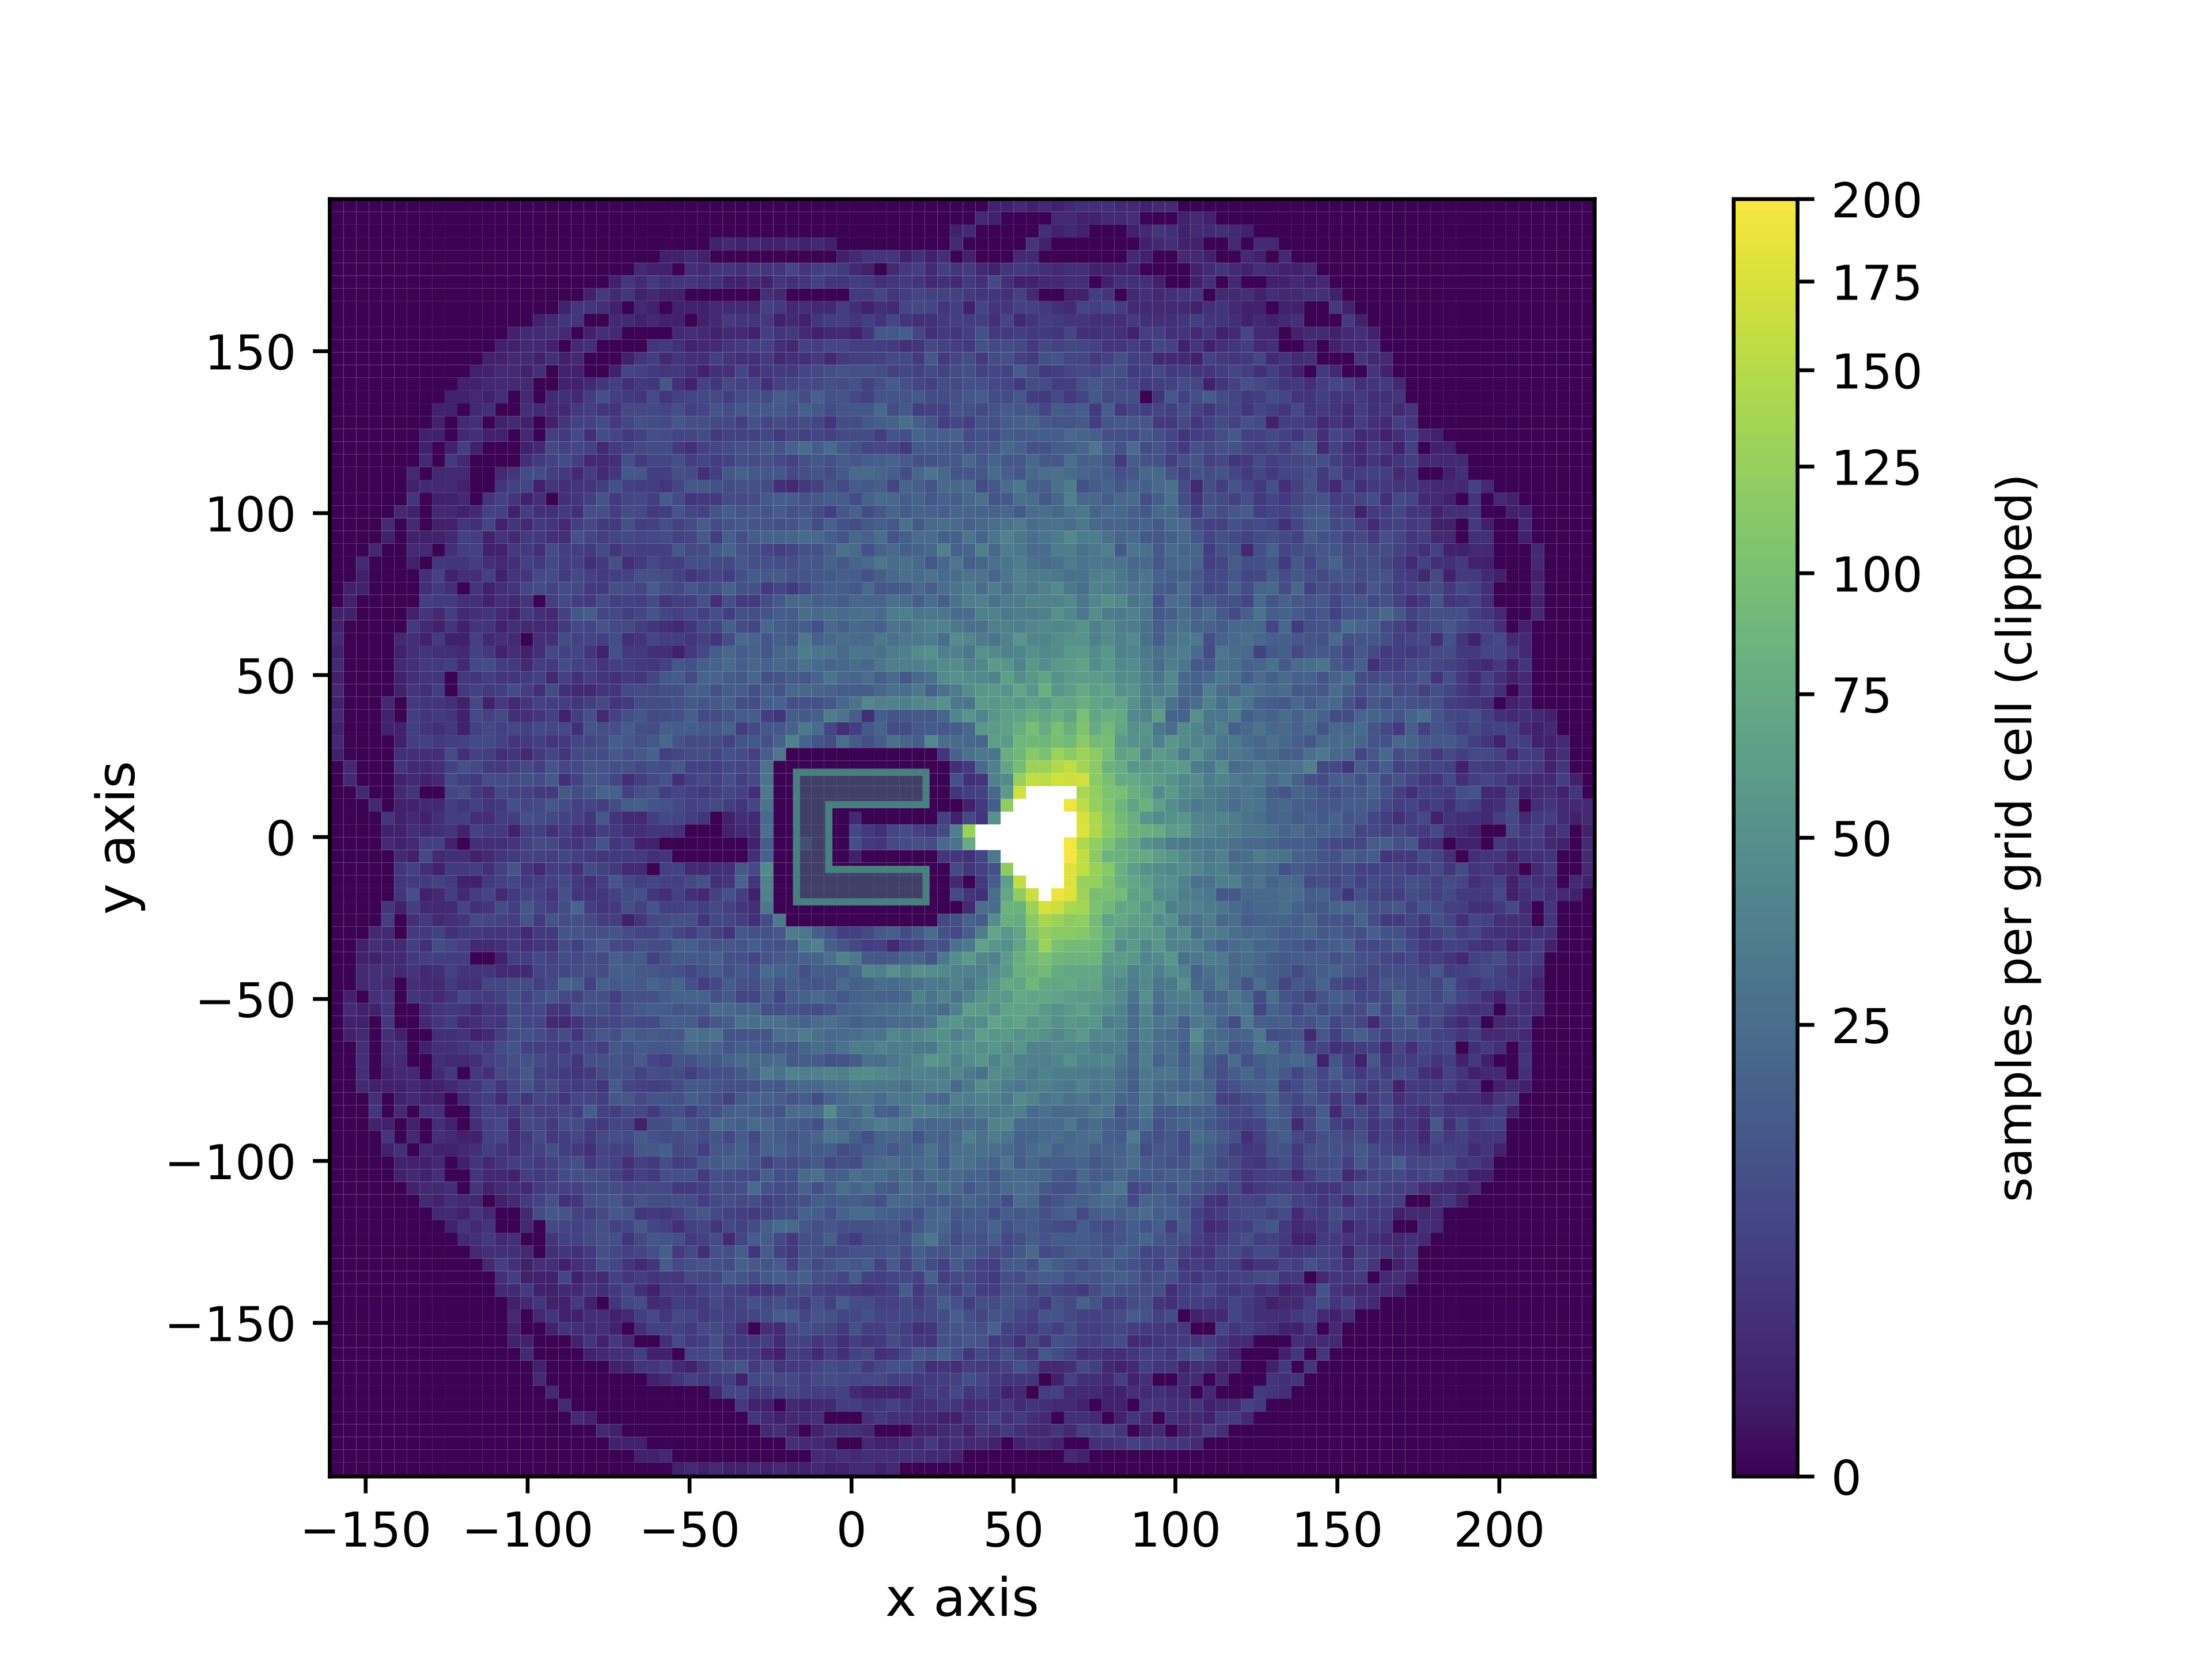
\includegraphics[width=.8\columnwidth]{dataset/monochromatic-omniscient/positions-heatmap}}
	\caption{Positions heatmap.}
	\label{fig:densisy-omniscient}
\end{figure}


\begin{figure}[htbp]
\centerline{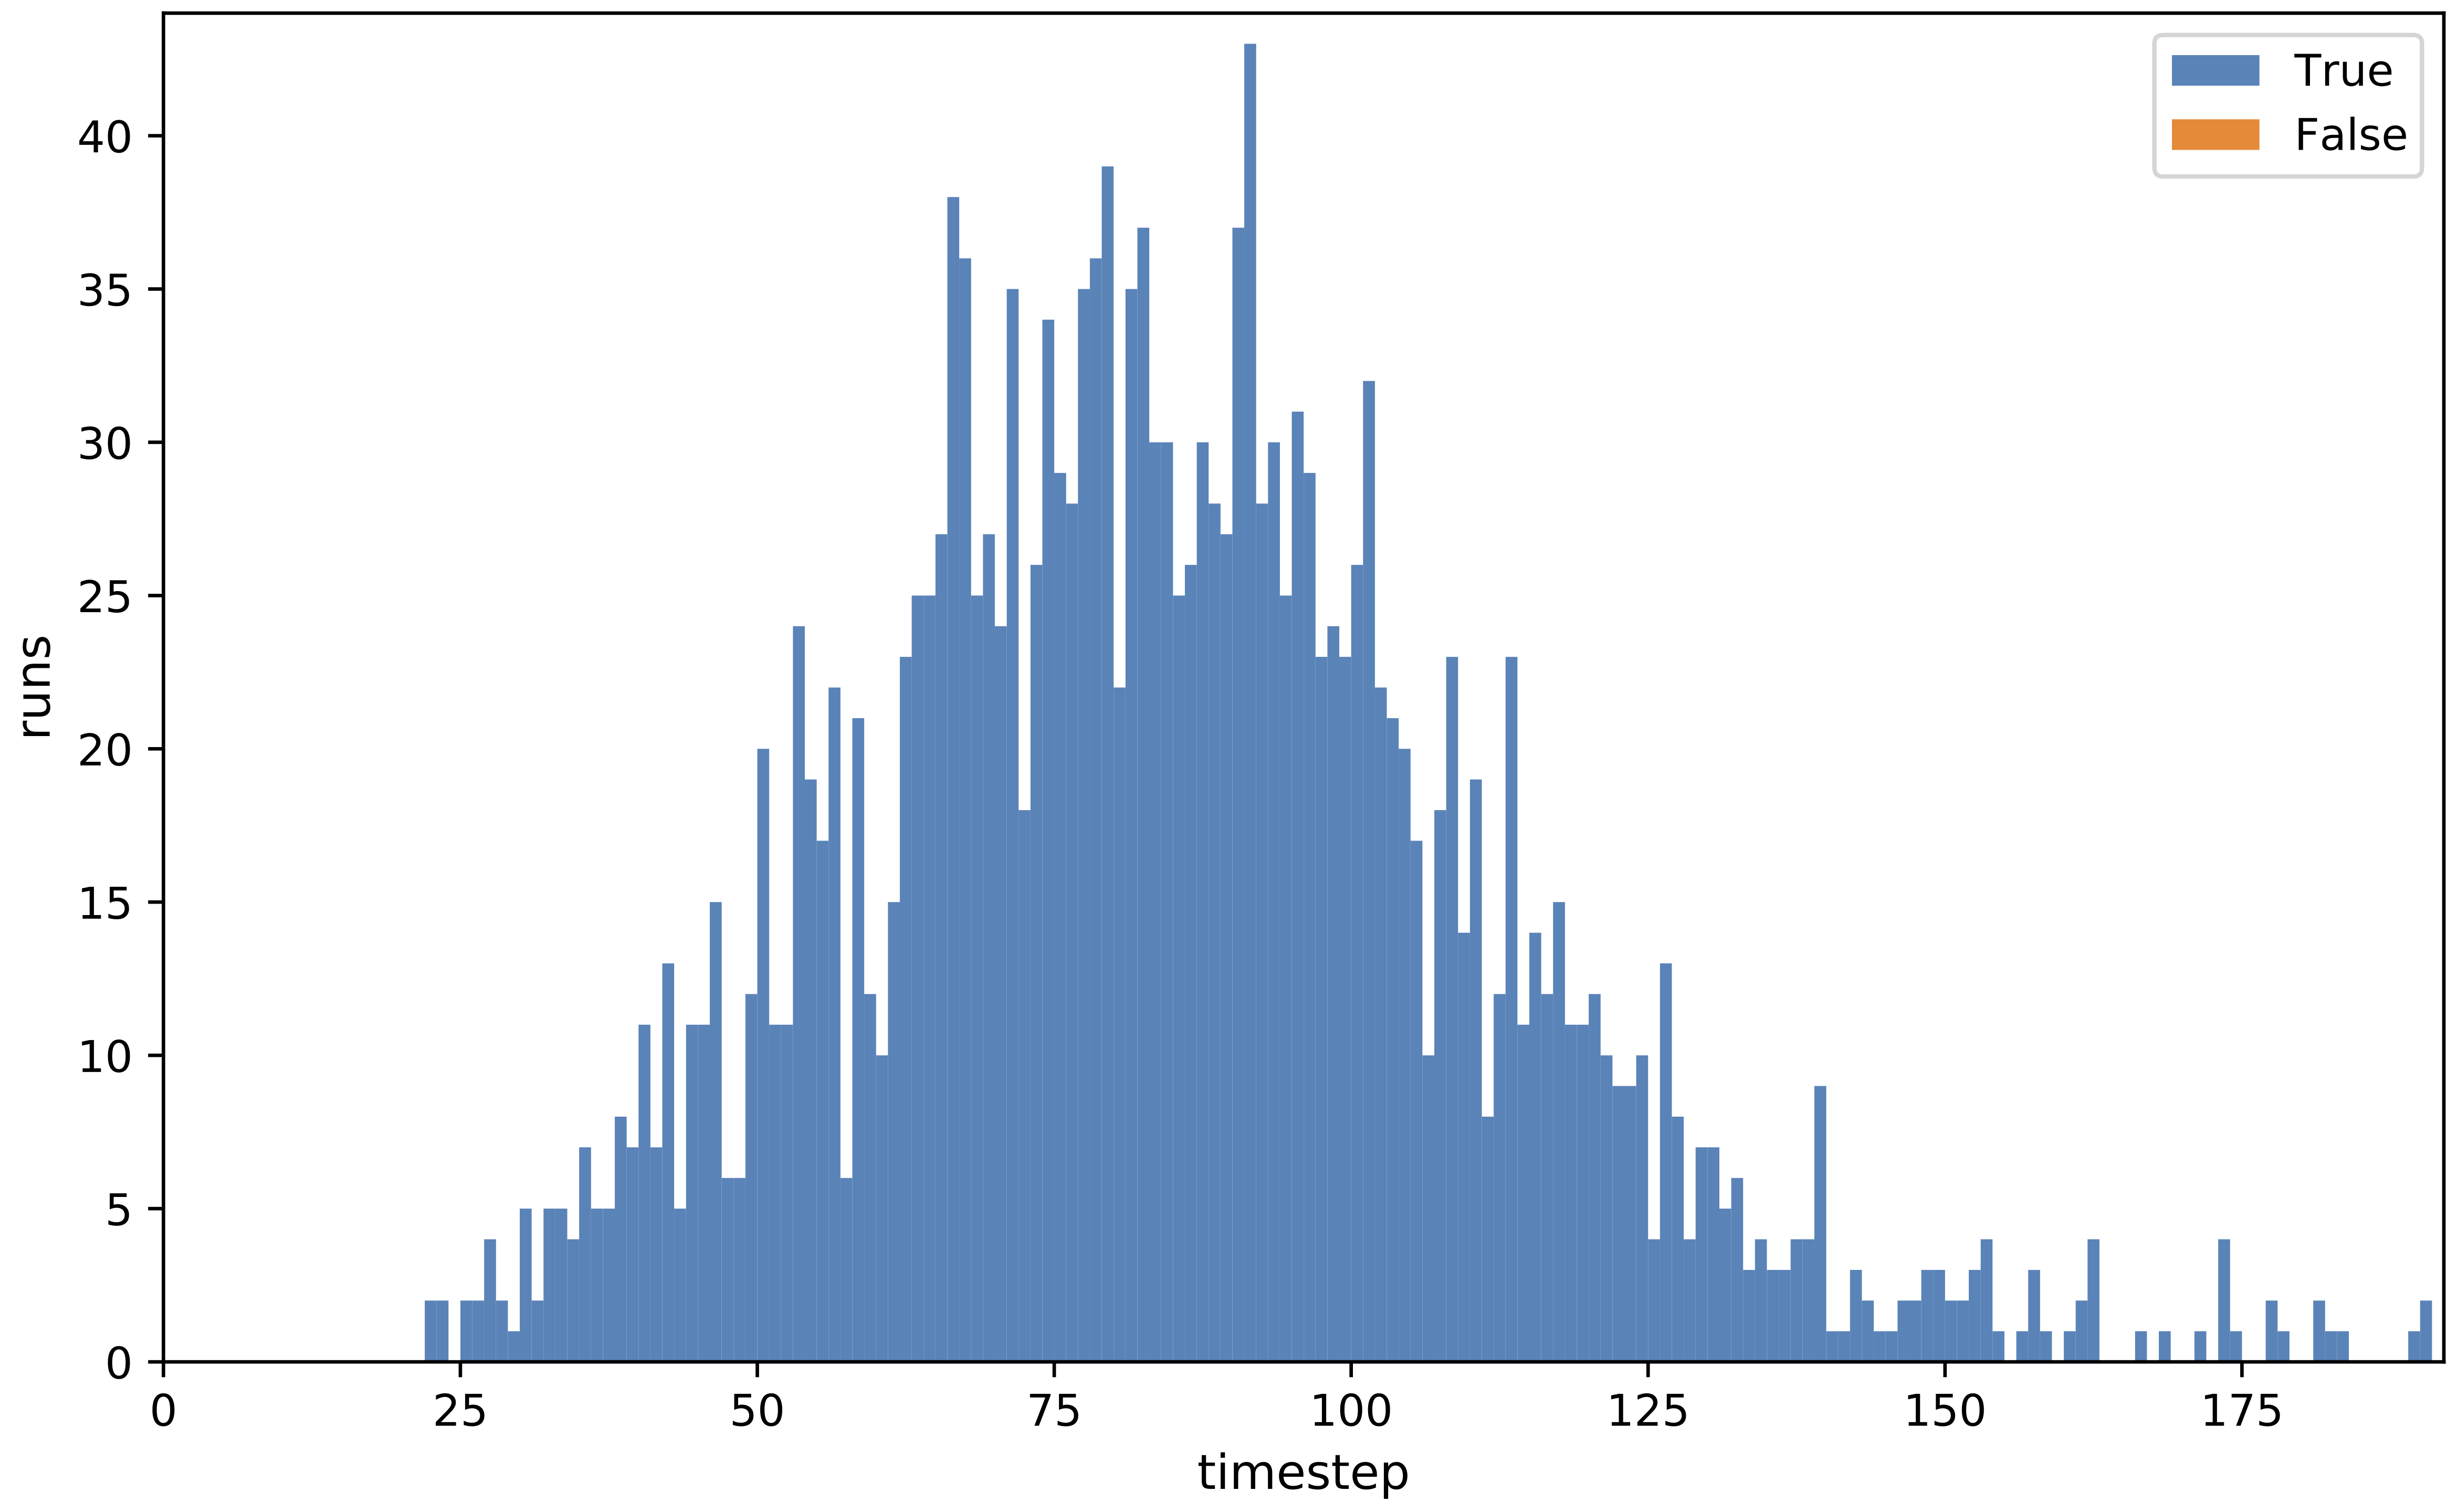
\includegraphics[width=.8\columnwidth]{dataset/monochromatic-omniscient/goal-reached}}
	\caption{Time to reach the goal.}
	\label{fig:goal-reached-omniscient}
\end{figure}

Plotting the position and orientation errors over time shows the convergence of 
the omniscient controller. In Figure \ref{fig:distance-from-goal-omniscient} 
are shown the euclidean distance and the angular difference between the pose of 
the robot and the goal pose over time. In Figure \ref{fig:pose-over-time} is 
instead shown the pose over time.

\begin{figure}[htbp]
	
\centerline{\includegraphics[width=\columnwidth]{dataset/monochromatic-omniscient/distances-from-goal}}
	\caption{Distance from goal over time.}
	\label{fig:distance-from-goal-omniscient}
\end{figure}

\begin{figure}[htbp]
	
\centerline{\includegraphics[width=.8\columnwidth]{dataset/monochromatic-omniscient/pose-over-time}}
	\caption{Distance from goal over time.}
	\label{fig:pose-over-time}
\end{figure}
